%%%%%%%%%%%%%%%%%%%%%%%%%%%%%%%%%%%%%%%%%%%%%%%%%%%%%%%%%%%%%%%%%%%%%%%%
% 
% This work is licensed under the Creative Commons
% Attribution-NonCommercial-ShareAlike 4.0 International License. To
% view a copy of this license, visit
% http://creativecommons.org/licenses/by-nc-sa/4.0/.
% 
% Portions of this work such as stylesheets and resource files may be
% subject to other licenses or terms.  Refer to those files or related
% documentation for additional information.
% 
%%%%%%%%%%%%%%%%%%%%%%%%%%%%%%%%%%%%%%%%%%%%%%%%%%%%%%%%%%%%%%%%%%%%%%%%

\documentclass[pdflatex,letterpaper,twoside,12pt]{book}

\title             {N4VEM Operations Manual}
\author            {Maintained by:\\Matt Kimball K4MTK\\Steve Crow KG4PEQ}
\date              {26-Apr-2013}
\newcommand\docver {Draft Version 19}

\def \logofile     {sty/arca_logo.jpg}

\usepackage{sty/arcabook}
\arcaFormat{printing}
\disableAutoNumbering
\useColorLinks

\printWatermark{DRAFT}

\begin{document}
\arcaTitlePage
\skipToTOC
\arcaTOC

%%%%%%%%%%%%%%%%%%%%%%%%%%%%%%%%%%%%%%%%%%%%%%%%%%%%%%%%%%%%%%%%%%%%%%%%
%%%%%%%%%%%%%%%%%%%%%%%%%%%%%%%%%%%%%%%%%%%%%%%%%%%%%%%%%%%%%%%%%%%%%%%%
%%%%%%%%%%%%%%%%%%%%%%%%%%%%%%%%%%%%%%%%%%%%%%%%%%%%%%%%%%%%%%%%%%%%%%%%
%%%%%%%%%%%%%%%%%%%%%%%%%%%%%%%%%%%%%%%%%%%%%%%%%%%%%%%%%%%%%%%%%%%%%%%%
%%%%%%%%%%%%%%%%%%%%%%%%%%%%%%%%%%%%%%%%%%%%%%%%%%%%%%%%%%%%%%%%%%%%%%%%
%%%%%%%%%%%%%%%%%%%%%%%%%%%%%%%%%%%%%%%%%%%%%%%%%%%%%%%%%%%%%%%%%%%%%%%%

\chapter{About this Manual}

\section{Introduction}

The ARCA Operations Manual was created to provide an overview of the functions of ARCA and Radio Amateur Civil Emergency Services (RACES) operations during the Response and Recovery phases of an emergency, disaster or other official activation.

This manual sets forth the fundamental operating theories which guide the entire ARCA team and also establishes specific policies that govern the operation of the team and its individual members.  It does not, however, dive into many detailed processes which are best left to separate training documents.  For example, this manual indicates the type of message traffic which will be handled by ARCA and its general flow, but does not provide specific steps involved in copying that traffic.

%%%%%%%%%%%%%%%%%%%%%%%%%%%%%%%%%%%%%%%%%%%%%%%%%%%%%%%%%%%%%%%%%%%%%%%%
%%%%%%%%%%%%%%%%%%%%%%%%%%%%%%%%%%%%%%%%%%%%%%%%%%%%%%%%%%%%%%%%%%%%%%%%

\section{How to Use this Manual}

This is a living document and will continue to evolve over time as ARCA grows as an organization.  All ARCA team members and Emergency Communications partners are encouraged to provide feedback on the content of this manual and make recommendations on ways the team can improve.  Please direct those suggestions to the ARCA Leadership Team.

Some changes to the core structure of ARCA must go through a specific approval process.  For example, they might need to be approved by the Virginia Department of Emergency Management (VDEM), or may need to be voted on by the membership.  However, the majority of what is contained in this manual can be fairly easily modified to suit the changing needs of the team.  All team members are encouraged to periodically review this manual, and the ARCA Leadership Team will make every effort to notify team members of any significant changes.

In most cases, this manual is updated to reflect the way we're already doing things, not to establish new policies or change our procedures.  Most of that is handled at meetings of the Leadership Team and the monthly membership meetings.

%%%%%%%%%%%%%%%%%%%%%%%%%%%%%%%%%%%%%%%%%%%%%%%%%%%%%%%%%%%%%%%%%%%%%%%%
%%%%%%%%%%%%%%%%%%%%%%%%%%%%%%%%%%%%%%%%%%%%%%%%%%%%%%%%%%%%%%%%%%%%%%%%

\section{Other Important Documents}

In addition to this Operations Manual, the Virginia Emergency Services Team (VEST) Standard Operating Procedure (SOP), Appendix F contains the ARCA SOP and contains other procedures and team information as filed with VDEM.

%%TODO:  Verify "Appendix F"

%%%%%%%%%%%%%%%%%%%%%%%%%%%%%%%%%%%%%%%%%%%%%%%%%%%%%%%%%%%%%%%%%%%%%%%%
%%%%%%%%%%%%%%%%%%%%%%%%%%%%%%%%%%%%%%%%%%%%%%%%%%%%%%%%%%%%%%%%%%%%%%%%

\section{Redistribution and Adaptations}

The ARCA Leadership Team has adopted a philosophy of sharing information with the amateur community.  Anything produced by ARCA which may be of benefit to the ham radio world is made available for distribution and adaptation in accordance with the Creative Commons license.  Please feel free to use this manual as the foundation for your own organization's operations.  We do ask that if you reuse portions of this manual or produce something significantly inspired by what you see here, that you not only reference this manual, but also let us know about it if you can:  we might be able to learn something from you!  That's why we share:  to learn from one another.

The general format and tone of this manual was adapted from the NWS Wakefield SKYWARN Amateur Radio Support Team Operations Manual, which is also published under a Creative Commons license.  It is available from http://www.wx4akq.org/.

%%%%%%%%%%%%%%%%%%%%%%%%%%%%%%%%%%%%%%%%%%%%%%%%%%%%%%%%%%%%%%%%%%%%%%%%
%%%%%%%%%%%%%%%%%%%%%%%%%%%%%%%%%%%%%%%%%%%%%%%%%%%%%%%%%%%%%%%%%%%%%%%%
%%%%%%%%%%%%%%%%%%%%%%%%%%%%%%%%%%%%%%%%%%%%%%%%%%%%%%%%%%%%%%%%%%%%%%%%
%%%%%%%%%%%%%%%%%%%%%%%%%%%%%%%%%%%%%%%%%%%%%%%%%%%%%%%%%%%%%%%%%%%%%%%%
%%%%%%%%%%%%%%%%%%%%%%%%%%%%%%%%%%%%%%%%%%%%%%%%%%%%%%%%%%%%%%%%%%%%%%%%
%%%%%%%%%%%%%%%%%%%%%%%%%%%%%%%%%%%%%%%%%%%%%%%%%%%%%%%%%%%%%%%%%%%%%%%%

\chapter{ARCA Basics}

\section{ARCA at a Glance}

The Virginia Department of Emergency Management (VDEM) Amateur Radio Communications Auxiliary was created in 2007 solely to provide emergency communications support to the Virginia Emergency Operations Center (VEOC).

ARCA remains operationally separate from other Emergency Communications (EMCOMM) organizations, such as ARES and SKYWARN, as well as the various clubs.  In order to function effectively, ARCA needs to maintain a close working relationship with all of its EMCOMM partners.  To do this, ARCA routinely participates in drills and other training activities with other groups and encourages all EMCOMM entities in Virginia to work together – amongst themselves and with ARCA – to continuously develop improved ways of doing things and to sharpen each others' skills.

From time to time, members of other EMCOMM groups may be invited to operate from the ARCA amateur radio station, N4VEM, and at all times, any licensed amateur radio operator, regardless of affiliation or license class, is welcome to drop in on the monthly membership meetings.  This will provide an ``inside look'' at why ARCA exists and how it operates, and will further strengthen the partnership between ARCA and the rest of the amateur radio community.  Information on how to attend a meeting as a non-member is provided later in this manual.

During formal activations of VEOC and ARCA, our team members man the radio room and provide ``last resort'' backup communications between VEOC and the many served agencies around the state, primarily local EOC's.  Our team members are trained in the handling of formal message traffic in the FEMA standard Incident Command System (ICS) format over a variety of communication channels including HF, VHF/UHF, and digital modes.

Messages properly received from a served agency are documented and relayed to the VDEM Watch Center, which will route the message further toward its destination within VEOC.  In the other direction, representatives of served agencies stationed inside VEOC may occasionally generate an outbound message to be delivered via amateur radio.  These messages are delivered to us by the VDEM Watch Center and are sent via the most expedient means possible.

The function of ARCA is to serve as a replacement for the telephone when all else has failed.  We typically don't run nets (other than for our own training purposes).  We never dictate how other EMCOMM groups work, aside from specifying how to communicate with us.  We try not to handle traffic that can be delivered by other means.  We are not intended as a means for staffing the local EOC's or other served agencies.  Bottom line:  we are the backup link between VEOC and the rest of the state.  That's it!  We do one thing, and we do it well!

%%%%%%%%%%%%%%%%%%%%%%%%%%%%%%%%%%%%%%%%%%%%%%%%%%%%%%%%%%%%%%%%%%%%%%%%
%%%%%%%%%%%%%%%%%%%%%%%%%%%%%%%%%%%%%%%%%%%%%%%%%%%%%%%%%%%%%%%%%%%%%%%%

\section{Purpose of ARCA}

ARCA exists to provide professional amateur radio communications in response to VEOC operational needs.  ARCA will have both operational and educational components and consist of volunteers who are amateur radio emergency communication volunteers.  All active personnel must hold an active FCC license.

%%%%%%%%%%%%%%%%%%%%%%%%%%%%%%%%%%%%%%%%%%%%%%%%%%%%%%%%%%%%%%%%%%%%%%%%
%%%%%%%%%%%%%%%%%%%%%%%%%%%%%%%%%%%%%%%%%%%%%%%%%%%%%%%%%%%%%%%%%%%%%%%%

\section{Inclusion and Non-Discrimination Policy}

ARCA has flourished by embracing the unique background and abilities of every team member.  Each individual brings a distinct skill set to the team and we must maintain an environment of inclusion and non-discrimination for all volunteers.  We welcome all participants who, with training and reasonable accommodation, can perform the basic functions required of a team member in their position, and we will seek out modified or alternative roles for other members where possible.

We do not tolerate abusive or discriminatory behavior based in whole or in part, on the person's race, color, national origin, age, religion, disability status, gender, sexual orientation, gender identity, veteran/military status, genetic information, or marital status.  While our resources are limited, we make every effort to extend reasonable accommodations to volunteers who may have special requirements during the training process and in the routine performance of SKYWARN functions.  These accommodations may include facility access considerations; transportation, seating, or dietary arrangements; accessibility devices; and modification of operating procedures as needed.

Requests for accommodation or concerns over potential violations of this policy may be directed to the appropriate member of the Leadership Team.

%%%%%%%%%%%%%%%%%%%%%%%%%%%%%%%%%%%%%%%%%%%%%%%%%%%%%%%%%%%%%%%%%%%%%%%%
%%%%%%%%%%%%%%%%%%%%%%%%%%%%%%%%%%%%%%%%%%%%%%%%%%%%%%%%%%%%%%%%%%%%%%%%

\section{Mission of ARCA}

The mission of ARCA is to develop and maintain the leadership and organizational structure necessary to provide radio communications support to community agencies and the people in and around the Commonwealth of Virginia whenever:

\begin{itemize}
	\item Conventional communications are inadequate to meet the public safety or humanitarian needs;
	\item Amateur radio resources may help facilitate response or recovery in any emergency situation;  
	\item Lives and property can be protected;
	\item Human suffering can be relieved;
	\item Amateur radio resources may help facilitate effective activities performed for the good of the general public;  
	\item It is necessary, under any and all circumstances, to ensure that no community goes without essential communication.
\end{itemize}

%%%%%%%%%%%%%%%%%%%%%%%%%%%%%%%%%%%%%%%%%%%%%%%%%%%%%%%%%%%%%%%%%%%%%%%%
%%%%%%%%%%%%%%%%%%%%%%%%%%%%%%%%%%%%%%%%%%%%%%%%%%%%%%%%%%%%%%%%%%%%%%%%

\section{ARCA Principles}

ARCA strives to enhance the reliability, quality, and professionalism of EMCOMM personnel by:

\begin{itemize}
	\item Establishing training and performance standards, policies and procedures; and
	\item Providing management and supervision of amateur radio operators registered with this Auxiliary that may be activated to provide communications on behalf of VDEM and the Commonwealth of Virginia requesting our assistance.
\end{itemize}

ARCA pledges a commitment to preparedness and service in protection of public health, safety and welfare by encouraging innovative leadership and individual responsibility which enhances the reliability and excellence of amateur radio emergency communications. We motivate amateur radio operators to excel in all facets of emergency communications and recognize those who exemplify our Emergency Communications (EMCOMM) philosophy.

%%%%%%%%%%%%%%%%%%%%%%%%%%%%%%%%%%%%%%%%%%%%%%%%%%%%%%%%%%%%%%%%%%%%%%%%
%%%%%%%%%%%%%%%%%%%%%%%%%%%%%%%%%%%%%%%%%%%%%%%%%%%%%%%%%%%%%%%%%%%%%%%%

\section{ARCA Values}

ARCA members reflect the following qualities and personal values:

\begin{enumerate}
	\item We are responsible and accountable;
	\item We demonstrate integrity and initiative;
	\item We are truthful and respectful of those we serve;
	\item We are, above all, dependable and trustworthy;
	\item We strive to maintain personal growth throughout all activities; and
	\item We are competent to perform our assigned duties and responsibilities.
\end{enumerate}

%%%%%%%%%%%%%%%%%%%%%%%%%%%%%%%%%%%%%%%%%%%%%%%%%%%%%%%%%%%%%%%%%%%%%%%%
%%%%%%%%%%%%%%%%%%%%%%%%%%%%%%%%%%%%%%%%%%%%%%%%%%%%%%%%%%%%%%%%%%%%%%%%

\section{Operational Objectives}

ARCA will aid in the passage of resource requests, damage assessments, situation reports, and other formal message traffic between VEOC and localities within the Commonwealth.   The auxiliary will supplement routine communications during exercises, declared or undeclared disasters, when augmented by VEOC, or at the request of other jurisdictions throughout the Commonwealth.

The Auxiliary will maintain a complete amateur station within the VEOC capable communicating with all jurisdictions within the Commonwealth, encompassing multiple bands and modes, and will ensure all operators are trained on the proper operation of these systems.

%%%%%%%%%%%%%%%%%%%%%%%%%%%%%%%%%%%%%%%%%%%%%%%%%%%%%%%%%%%%%%%%%%%%%%%%
%%%%%%%%%%%%%%%%%%%%%%%%%%%%%%%%%%%%%%%%%%%%%%%%%%%%%%%%%%%%%%%%%%%%%%%%

\section{Leadership Team}

ARCA is not a club, however, a portion of its organizational structure does resemble a traditional amateur radio club, and we do have a group of elected officials who work alongside a handful of folks appointed to their position either internally or by the Commonwealth.  Collectively, this is the ARCA Leadership Team.

While each position on the Leadership Team does have its own unique responsibilities, it's important to understand that all members of the Leadership Team share an equal responsibility for the smooth operation of ARCA.  Everyone on the Leadership Team is receptive to the feedback of our team members and as a member of ARCA you should feel comfortable approaching anyone on the Leadership Team with questions, suggestions, or concerns.

In addition to the formal Leadership Team, there are always a number of projects going on.  Things like working out communication plans with certain parts of the state, planning team activities and training events, or even maintaining this manual.  We call these workgroups.  They are a great way to tap into the specialized talents of small groups of ARCA team members.  As various and sundry projects come up, please volunteer to help where you can.  Feel free to ``take the bull by the horns'' and lead one of those teams.  It takes many hands to run ARCA and the leadership can't do it all.

\subsection{Overview of the Leadership Team}

There are two types of officers in ARCA.  Elected officers are selected and voted in by the ARCA membership.  With few rare exceptions, all ARCA members in good standing are both eligible and encouraged to run for one of these spots when one opens up.  Appointed officers hold an ex officio position (meaning they are a member by virtue of holding some other office).  Appointed officers typically serve longer terms than elected officers, and generally have no specific term limit, however, they also do not have voting privileges and cannot serve as elected officers.

The Leadership Team and its officers are responsible for setting the overall strategy for ARCA and also lead efforts to update this manual as will occasionally be needed.  Together, the Leadership Team is responsible for ensuring ARCA remains both qualified and fully prepared to meet the EMCOMM needs of the Commonwealth.

The elected officers of ARCA are the President, Vice-President, Recording Secretary, and Technical Secretary.  Appointed officers are the VDEM Amateur Radio Liaison and State RACES Officers.

The next few sections will provide a general overview of the key functions of each of the positions on the Leadership Team.  Again, all members of the Leadership Team share an equally important responsibility for the direction of the ARCA organization.  No one position is more or less important than any other, and no single person is ``in charge'' of ARCA.

\subsection{President}

The President presides over all regular and special meetings of ARCA.  They work with the VDEM Amateur Radio Liaison to develop and maintain the operating procedures for the VDEM amateur radio station.  All formal ARCA committees are appointed by the President, who is automatically a member of those committees.  At the request of the VDEM Amateur Radio Liaison, the President may call special meetings of ARCA as may occasionally be needed.  The President has the authority to appoint positions if and when needed to conduct official ARCA business.

\subsection{Vice President}

The Vice President works hand-in-hand with the President and VDEM Amateur Radio Liaison to develop and maintain the operating procedures for the VDEM amateur radio station. They are also responsible for any duties assigned by the President.

If the President is absent or unable to fulfill their duties, the Vice President assumes those roles.

\subsection{Secretary}

The role of the Secretary is to keep accurate minutes of all ARCA meetings and notify ARCA membership of upcoming meetings.  These notifications are usually sent via e-mail or some other electronic notification system.  Meetings are typed up, printed, and distributed at the following month's membership meeting, and are archived for posterity.

\subsection{Technical Secretary}

The Technical Secretary prepares written recommendations for repair, replacement, and general operation of the VDEM amateur radio station and its equipment, and submits that information to the VDEM Amateur Radio Liaison.  They also make recommendations relating to the operating procedures for the VDEM amateur radio station based on operating experience and equipment availability.  Finally, they catalog and maintain manuals for all of the equipment used in the VDEM amateur radio station, and keep that information on file with the VDEM Amateur Radio Liaison.

\subsection{VDEM Amateur Radio License Trustee}

The VDEM Amateur Radio License Trustee holds legal responsibility for all amateur radio licenses used by the VDEM amateur radio station (N4VEM) and is the FCC point of contact with regard to VDEM licenses and operations.  They ensure that the station is maintained and operated in compliance with FCC Part 97 at all times, and are personally and officially responsible for answering inquiries from the public and the FCC regarding the operation of the station.  All use of VDEM amateur radio call signs must take place based on the direction of the Trustee.

The License Trustee is appointed by the Leadership Team from among the General Membership.  From a policy perspective, there is no minimum or maximum amount of time a member may serve as the License Trustee.  In practice, a new License Trustee may be selected as often as needed based on the needs of ARCA and VDEM.

\subsection{VDEM Amateur Radio Liaison}

The VDEM Amateur Radio Liaison provides VDEM policy guidance to ARCA through the State RACES Officer when RACES has been activated for emergency response. The VDEM Amateur Radio Liason provides coordination and guidance for recruitment, training, and assignment of duties in support of the VDEM mission and ARCA's objectives and purpose.

% \subsection{State RACES Officer}
% 
% The State RACES Officer's role in ARCA during a RACES activation, is to supervise operational activities along side of the VDEM Amateur Radio Liason, coordinate emergency communications and requests from within the Commonwealth of Virginia for amateur radio resources that may be needed to augment local resources.
% 
% \subsection{Assistant State RACES Officer}
% 
% The Assistant State RACES Officer fills the role of the State RACES Officer in the event they are unavailable.

%%%%%%%%%%%%%%%%%%%%%%%%%%%%%%%%%%%%%%%%%%%%%%%%%%%%%%%%%%%%%%%%%%%%%%%%
%%%%%%%%%%%%%%%%%%%%%%%%%%%%%%%%%%%%%%%%%%%%%%%%%%%%%%%%%%%%%%%%%%%%%%%%
%%%%%%%%%%%%%%%%%%%%%%%%%%%%%%%%%%%%%%%%%%%%%%%%%%%%%%%%%%%%%%%%%%%%%%%%
%%%%%%%%%%%%%%%%%%%%%%%%%%%%%%%%%%%%%%%%%%%%%%%%%%%%%%%%%%%%%%%%%%%%%%%%
%%%%%%%%%%%%%%%%%%%%%%%%%%%%%%%%%%%%%%%%%%%%%%%%%%%%%%%%%%%%%%%%%%%%%%%%
%%%%%%%%%%%%%%%%%%%%%%%%%%%%%%%%%%%%%%%%%%%%%%%%%%%%%%%%%%%%%%%%%%%%%%%%

\chapter{ARCA Membership}

There are three types of ARCA membership:  General, Support, and Appointed.  The most widely held form of membership is General Membership, which is available to anyone holding an amateur radio license of any class.  General Members vote on policies, procedures, elected officers, and a number of other topics, and are expected to attend membership meetings and participate in training exercises.

Appointed Memberships are extended to the VDEM Amateur Radio Liaison, the State RACES Officers, and those deemed necessary by the ARCA Leadership Team.

Support Members may or may not have a valid amateur radio license.  These are usually members who have expressed interest in supporting the operations of ARCA by helping with equipment maintenance or providing some other specialized service, but who do not wish to be included in the call-up list for ARCA activations.  Support Members are non-voting members.

General Membership requires the submission of an application and a vote of approval from the rest of the General Membership.  Support Members can join by contacting any member of the ARCA Leadership Team and completing an application form.  A move from Support Member to General Membership requires a vote of approval from the rest of the General Membership.

\section{Maintaining Active General Membership}

The success of ARCA depends on having a sufficiently large pool of active team members who regularly attend membership meetings and training exercises, and who are also available and willing to help man the ARCA Radio Room during formal activations.

In a perfect world, every team member would attend every meeting, participate in every training exercise, and show up for a shift during every activation.  We realize that's not practical.  By becoming an ARCA member, there is a minimum standard of participation to remain in General Membership status and retain voting privileges within ARCA.

At a minimum, team members should be able to commit to one membership meeting per calendar quarter, and should be able to participate in one training exercise or formal activation every six months.  Attendance will be taken at these events and it is each member's responsibility to make sure their participation is noted.

%%TODO:  Who maintains these records?

Falling behind on this minimum standard does not mean an automatic removal from the General Membership roster.  Team members will be given a three month window to come back to a monthly membership meeting and participate in a training exercise or activation before action is taken.  The minimum training and activation participation requirement won't apply if fewer than four training opportunities or activations have occurred in the previous six months.

Team members who do remain below the minimum standard will not be removed from ARCA.  Rather, they will be moved to a Support Membership role which removes them from the call-up list.  Members are reminded that Support Members do not have voting privileges and are not considered part of the General Membership.  To maintain a vote in ARCA affairs, the minimum participation standard must be met.

In all instances, the ARCA Leadership Team is able to make exceptions to individuals based on special circumstances such as health or transportation issues.

%%%%%%%%%%%%%%%%%%%%%%%%%%%%%%%%%%%%%%%%%%%%%%%%%%%%%%%%%%%%%%%%%%%%%%%%
%%%%%%%%%%%%%%%%%%%%%%%%%%%%%%%%%%%%%%%%%%%%%%%%%%%%%%%%%%%%%%%%%%%%%%%%

\section{Planning to Support ARCA}

When you consider becoming an ARCA member, please be sure to talk about it with your employer.  Some ARCA activities - both training and activations - take place on weekdays and may overlap with your normal working hours.  Let your supervisor know that you are filling an important role in the emergency preparedness of the Commonwealth of Virginia, and that an ability to participate in training and activations will be essential.  Discuss the fact that it may be necessary to take a day off a few times a year to train or to operate the radio desk.

If your employer has questions about your obligations as an ARCA member, feel free to put them in contact with a member of the ARCA Leadership Team.  We will be happy to explain what we do and how important it is to the citizens of Virginia.  If needed, ARCA leadership can provide documentation to your employer to verify your participation in a training exercise or activation at the conclusion of that event.

Along those same lines, please give careful consideration to any conflicts that might arise from your participation in both ARCA and another EMCOMM group such as ARES or SKYWARN.  It's not uncommon for two EMCOMM teams to be fighting for help from the same pool of volunteers during a major event.  We are by no means trying to discourage you from getting involved in multiple EMCOMM programs, but we do have to urge you to consider how you will balance your obligations to both organizations.

If you are going to be juggling a job and/or another EMCOMM team along with ARCA, you are ultimately responsible for ensuring that ARCA does not adversely interfere with your other obligations, and vice-versa.  If you suspect there may be a conflict, we will be happy to have you on our team as a Support Member.

%%%%%%%%%%%%%%%%%%%%%%%%%%%%%%%%%%%%%%%%%%%%%%%%%%%%%%%%%%%%%%%%%%%%%%%%
%%%%%%%%%%%%%%%%%%%%%%%%%%%%%%%%%%%%%%%%%%%%%%%%%%%%%%%%%%%%%%%%%%%%%%%%
%%%%%%%%%%%%%%%%%%%%%%%%%%%%%%%%%%%%%%%%%%%%%%%%%%%%%%%%%%%%%%%%%%%%%%%%
%%%%%%%%%%%%%%%%%%%%%%%%%%%%%%%%%%%%%%%%%%%%%%%%%%%%%%%%%%%%%%%%%%%%%%%%
%%%%%%%%%%%%%%%%%%%%%%%%%%%%%%%%%%%%%%%%%%%%%%%%%%%%%%%%%%%%%%%%%%%%%%%%
%%%%%%%%%%%%%%%%%%%%%%%%%%%%%%%%%%%%%%%%%%%%%%%%%%%%%%%%%%%%%%%%%%%%%%%%

\chapter{Meetings}

\section{Membership and Leadership Team Meetings}

Membership meetings are held monthly, generally on the third Wednesday of each month at 7:00 PM.  Meetings are on the floor of VEOC, which is under the Virginia State Police headquarters on Midlothian Turnpike.  Membership meetings are open to all ARCA members, regardless of membership type, though voting is limited to General Members.  Additionally, any interested members of the amateur radio community are invited to attend, but because of the secure nature of the facility, that visit will need to be pre-arranged to allow access.

Sometimes it will be necessary to reschedule a meeting, for example, if VEOC is active, or if a meeting date lands on or near a major holiday like Thanksgiving or Christmas.  Meeting reminders will be sent via e-mail a few days before each meeting, but non-members who are coming to our meeting should verify the meeting date and time with their contact a few days ahead of time.

Leadership Team meetings are held as needed and provide an opportunity for the elected and appointed members of the Leadership Team to come together, discuss matters relating to ARCA, special projects, initiatives, and policy changes.  These meetings may periodically include representatives of ARCA workgroups and active membership is encouraged to attend.  The date, time, and location of these meetings will vary.

%%%%%%%%%%%%%%%%%%%%%%%%%%%%%%%%%%%%%%%%%%%%%%%%%%%%%%%%%%%%%%%%%%%%%%%%
%%%%%%%%%%%%%%%%%%%%%%%%%%%%%%%%%%%%%%%%%%%%%%%%%%%%%%%%%%%%%%%%%%%%%%%%

\section{Attending Membership Meetings as a Guest}

All membership meetings are open to the general amateur radio community.  However, since the meeting location is a secure, restricted-access facility, coming to a meeting is not quite as easy as simply showing up.

If you are not a member of ARCA but you know someone who is, you are welcome to come along with them to the membership meeting.  There is no need to call ahead or make special arrangements.  Their credentials will open the gate for one vehicle only, so it will be easiest if you ride in together.  They can also get you into the building, walk you through signing in, and introduce you to the rest of the group.  They will need to escort you through the building, so do not leave their side.

If you don't know another ARCA member or can't travel to the EOC with them, please contact any member of the ARCA Leadership Team at least 48 hours in advance.  You will be provided with instructions on parking and how to request access to the parking lot if needed, and how to arrange for entry into the building once you're at VEOC.  You cannot simply drive up, punch in a code, and ask to be let in.  We need to communicate your information to the Virginia State Police ahead of time, otherwise you will experience a potentially lengthy delay while the VSP officer makes phone calls to try to identify you, and you may simply be denied access.

Do not be intimidated by the security and the extra steps needed to gain access to our meetings.  These are not restrictions we have put in place to discourage anyone from joining us.  If you have any questions at all, please reach out to the Leadership Team or any ARCA member.  We look forward to meeting you!

\arcabox{Helpful Tip}{Take a moment to review the ``VEOC Policies and Procedures'' section in this manual to make sure you know the basic rules of conduct while visiting our facility.}

%%%%%%%%%%%%%%%%%%%%%%%%%%%%%%%%%%%%%%%%%%%%%%%%%%%%%%%%%%%%%%%%%%%%%%%%
%%%%%%%%%%%%%%%%%%%%%%%%%%%%%%%%%%%%%%%%%%%%%%%%%%%%%%%%%%%%%%%%%%%%%%%%

\section {Attending Leadership Team Meetings as a Guest}

In general, Leadership Team meetings will be open to the general membership, and members are welcome to attend and participate.  There may be certain situations where the Leadership Team needs to discuss sensitive matters.  The President or Vice President may decide that one or more portions of a Leadership Team meeting is ``closed'' and attendance will be limited to the Leadership Team and certain other participants as needed.  Additionally, an entire meeting could be arranged as a closed session.

Persons wishing to attend Leadership Team meetings should contact the President and/or Vice President as far in advance as possible, since the date, time, and location of Leadership Team meetings may vary.

%%%%%%%%%%%%%%%%%%%%%%%%%%%%%%%%%%%%%%%%%%%%%%%%%%%%%%%%%%%%%%%%%%%%%%%%
%%%%%%%%%%%%%%%%%%%%%%%%%%%%%%%%%%%%%%%%%%%%%%%%%%%%%%%%%%%%%%%%%%%%%%%%

\section{Facility Map}

For your convenience in navigating to the VEOC Entrance, here is an aerial map from Google:

\begin{figure}[h!]
  \centering
  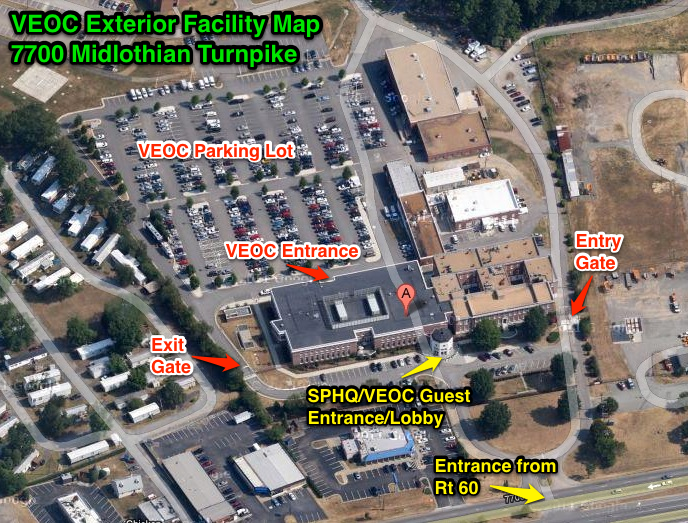
\includegraphics[width=\textwidth,keepaspectratio=true]{resources/veoc_map}
  \caption{Map of SPHQ and VEOC.\label{fig:ops-main-screen}}
\end{figure}

The address is 7700 Midlothian Turnpike, Richmond.

%%%%%%%%%%%%%%%%%%%%%%%%%%%%%%%%%%%%%%%%%%%%%%%%%%%%%%%%%%%%%%%%%%%%%%%%
%%%%%%%%%%%%%%%%%%%%%%%%%%%%%%%%%%%%%%%%%%%%%%%%%%%%%%%%%%%%%%%%%%%%%%%%
%%%%%%%%%%%%%%%%%%%%%%%%%%%%%%%%%%%%%%%%%%%%%%%%%%%%%%%%%%%%%%%%%%%%%%%%
%%%%%%%%%%%%%%%%%%%%%%%%%%%%%%%%%%%%%%%%%%%%%%%%%%%%%%%%%%%%%%%%%%%%%%%%
%%%%%%%%%%%%%%%%%%%%%%%%%%%%%%%%%%%%%%%%%%%%%%%%%%%%%%%%%%%%%%%%%%%%%%%%
%%%%%%%%%%%%%%%%%%%%%%%%%%%%%%%%%%%%%%%%%%%%%%%%%%%%%%%%%%%%%%%%%%%%%%%%

\chapter{General VEOC Policies and Procedures}

\section{Access Control, Badges, and Authorized Areas}

Access to VEOC facilities is controlled with electronic badges.

All registered members of ARCA are provided an official VDEM/VEST credentials for access to VEOC.  Members need to have their photo taken and will be required to provide personal information to VDEM to allow the badge to be produced.

These badges utilize a Radio Frequency Identifier (RFID) chip embedded within the card.  Card readers are installed at the perimeter of the parking lot and building, and at most doors and hallways.  Team members need to use their own badge for access.  Never allow anyone else to enter an area using your badge unless they are your guest and you are escorting them.  You are personally responsible for anyone who uses your badge!

\subsection{Using the Badge}

To activate the card reader, simply place the badge within an inch or two of the front of the card reader.  You will hear a faint beep or click, or will see a light to indicate the badge bas been read.  You may need to wave the badge back and forth slowly a couple of times to activate the reader.  If the area you are trying to access is not unlocked at that point, you may not be authorized for access to that area.

When it comes to finding out where you can and can't go in the facility, here are three good rules of thumb to remember:  If there's no other way you can get where you need to go, it's probably okay.  If you're not sure, stay out.  If it involves walking through the Watch Center, find another route!  Do not attempt to open any doors just to see if you can get in, and don't go into any offices or walk through any areas you don't absolutely have to access.

\subsection{Displaying Badges}

Badges must be worn above the waist with the photo clearly visible at all times while at VEOC.  While off VEOC property, badges are not to be displayed and should be kept in a secure location.

\subsection{Replacement of Badges}

You must report a lost or stolen badge to any member of the ARCA Leadership Team immediately.  Remember that you are responsible for all activity on your badge.  We will notify VDEM and have the badge terminated, and will assist you with obtaining a replacement  badge.

If you experience any problems with your badge, contact any member of the ARCA Leadership Team for assistance.  Please note that these badges do expire.  Be mindful of your expiration date and notify someone from the Leadership Team a couple months beforehand so that we may begin the process of having the badge renewed or reissued.

\subsection{Badge Restrictions}

For various legal and technical reasons, the VEST badges issued to ARCA team members have the word ``Employee'' on them.  You are reminded that these badges are not an employee identification badge and do not create any employment relationship between you and the Commonwealth of Virginia, and any attempt to use the badge for those purposes will result in revocation of the badge.

%%%%%%%%%%%%%%%%%%%%%%%%%%%%%%%%%%%%%%%%%%%%%%%%%%%%%%%%%%%%%%%%%%%%%%%%
%%%%%%%%%%%%%%%%%%%%%%%%%%%%%%%%%%%%%%%%%%%%%%%%%%%%%%%%%%%%%%%%%%%%%%%%

\section{When to Come to VEOC}

As long as you are a credentialed ARCA member, you do not need to call ahead for access to VEOC for monthly membership meetings, pre-arranged training exercises, or other such activities, unless you plan to arrive considerably before the start of the event (more than 30 minutes early).

If VEOC is activated, do not self-deploy!  Follow the established call-up procedures to respond to volunteer requests and wait for your offer to be acknowledged.  Members who show up unannounced will be turned away and may be subject to additional action.  If you have volunteered and been accepted for a shift, try to arrive 30 minutes early to get checked in and get situated in the radio room.

%%%%%%%%%%%%%%%%%%%%%%%%%%%%%%%%%%%%%%%%%%%%%%%%%%%%%%%%%%%%%%%%%%%%%%%%
%%%%%%%%%%%%%%%%%%%%%%%%%%%%%%%%%%%%%%%%%%%%%%%%%%%%%%%%%%%%%%%%%%%%%%%%

\section{Dress Code}

The dress code for all activities at VEOC is quite simple:  be presentable.  We do have a limited number of official VEST shirts available but you will need to request one well ahead of time.  If you have a VEST shirt, wear that, along with neat and clean pants (jeans or khakis are okay).  If you do not have a VEST shirt, most any polo shirt will do.  Avoid t-shirts and shorts if at all possible.

Keep in mind that during VEOC activations, a number of local and state officials may be present in the EOC, including local media and the Governor!  Please be prepared to project a positive image of amateur radio and the ARCA team by dressing appropriately.

%%%%%%%%%%%%%%%%%%%%%%%%%%%%%%%%%%%%%%%%%%%%%%%%%%%%%%%%%%%%%%%%%%%%%%%%
%%%%%%%%%%%%%%%%%%%%%%%%%%%%%%%%%%%%%%%%%%%%%%%%%%%%%%%%%%%%%%%%%%%%%%%%

\section{Guests}

You are welcome to bring guests to monthly membership meetings.  Guest access to VEOC during activations will be at the discretion of the VDEM Amateur Radio Liaison Officer.

%%%%%%%%%%%%%%%%%%%%%%%%%%%%%%%%%%%%%%%%%%%%%%%%%%%%%%%%%%%%%%%%%%%%%%%%
%%%%%%%%%%%%%%%%%%%%%%%%%%%%%%%%%%%%%%%%%%%%%%%%%%%%%%%%%%%%%%%%%%%%%%%%

\section{Parking}

The VEOC parking lot is located behind the Virginia State Police Administrative Headquarters (SPHQ) and is a controlled-access lot.  When arriving at SPHQ, enter through the gate to the right-hand side of the building.  Wave your badge over the card reader and wait for the green light.  You may have to wave it several times to activate the reader.  There is a second reader several feet up above the first one that sometimes works better.

If your badge does not read, follow the instructions printed next to the numeric keypad to call the VSP Duty Officer and request access.  Identify as a ham radio volunteer needing to access the EOC and provide your name.  Your identity will be checked against a list of ARCA team members authorized for access to the facility.  If you cannot be authenticated (for example, if you have self-deployed and we are not expecting you) your access will be denied.

Remember to wait for the green light before passing through the gate.  No tailgating!  You must scan your badge and wait for the green light before passing through the gate!

When you arrive, go to the bottom of the hill, make a left, and swing around to the back of the back side of the EOC.  There is a large parking lot.  Pick any space except for those marked “Reserved for VDEM.”  Remember to secure any valuables and lock your vehicle.  Drive slowly and exercise extreme caution maneuvering around the building at the bottom of the hill as there is a blind spot.

The entrance to VEOC is down the stairs next to the sign referencing the ``Emergency Operations and Fusion Center.''  Use your badge or the doorbell to gain access.

%%%%%%%%%%%%%%%%%%%%%%%%%%%%%%%%%%%%%%%%%%%%%%%%%%%%%%%%%%%%%%%%%%%%%%%%
%%%%%%%%%%%%%%%%%%%%%%%%%%%%%%%%%%%%%%%%%%%%%%%%%%%%%%%%%%%%%%%%%%%%%%%%

\section{Checking In and Out}

When you first come in to the building you will need to sign in, even if you are a credentialed ARCA member.  This sign-in sheet is not so much a form of access control as it is a way to maintain a head count of people inside the building in case of an emergency.

If VEOC is not active – for example, during our regular monthly membership meetings – there will be a book on the counter next to the clock.  You will be asked for your name, affiliation (that's ``ARCA''), and arrival time in 24-hour format.  You will also need to note your departure time when you leave.  If you're just going to run out to your vehicle and grab something, it's usually not necessary to sign out and back in.  However, if you are leaving the parking lot, you must sign out.

If VEOC is active, an officer will typically be stationed at a table with a sign-in book.  The book is organized by Emergency Support Function (ESF).  There is a section for ARCA, usually toward the beginning of the book.  The officer will be happy to help you locate the appropriate section and get signed in.  If your name is not on the list, just add it to the space at the bottom.  You will also need to note your departure time when you leave.  If you need to briefly leave the building to grab something from your vehicle, check with the officer to see if you need to sign out and back in.  If you are leaving the parking lot, definitely sign out.

Regardless of VEOC activity, if you are the first person to arrive at the radio room, step into the VEOC Watch Center and check in with any of the VDEM employees.  Quickly introduce yourself and let them know you will be in the radio room.  If you are expecting others, let them know how many and when, if you have that information.  Likewise, if you are the last person out, check in with a VDEM employee in the Watch Center and let them know all ham radio personnel have left.

%%%%%%%%%%%%%%%%%%%%%%%%%%%%%%%%%%%%%%%%%%%%%%%%%%%%%%%%%%%%%%%%%%%%%%%%
%%%%%%%%%%%%%%%%%%%%%%%%%%%%%%%%%%%%%%%%%%%%%%%%%%%%%%%%%%%%%%%%%%%%%%%%

\section{Personal Items}

You should only bring the minimum amount of personal items required to support your stay in the radio room.  Space is extremely limited and no lockers are available.

There should be no need to bring any radios (other than an HT for on-site comms use or temporary communications in the event of an evacuation), computers, or other equipment with you.  It is acceptable to bring a tablet or laptop with you if you prefer to use your own equipment.  However, do be aware that there will be significant limits on both the amount of space and technical support available should you choose to supply your own computing gear.

Do not bring backpacks or large bags of stuff into the radio room with you.  All bags are of course subject to search upon entry to the facility and at any other point, but the primary concern is available space: we don't have any!  If you don't absolutely need to have it with you, leave it in your vehicle.

%%%%%%%%%%%%%%%%%%%%%%%%%%%%%%%%%%%%%%%%%%%%%%%%%%%%%%%%%%%%%%%%%%%%%%%%
%%%%%%%%%%%%%%%%%%%%%%%%%%%%%%%%%%%%%%%%%%%%%%%%%%%%%%%%%%%%%%%%%%%%%%%%

\section{Food and Drinks}

There is a small refrigerator in the kitchen which can be used to store a few cans of soda, some sandwiches, etc. if desired.  If you bring it, write your name on it clearly.  Remember to take home anything you don't consume while you're there.

During lengthy VEOC activations, breakfast, lunch, and dinner are typically provided by VDEM, and a supply of cold beverages will generally remain available in the kitchen adjacent to the floor of the EOC.  However, you should come prepared with snacks and a few beverages of your own, particularly if you have special dietary needs.

Coffee is always available for brewing, however, donations (in the receptacle provided) are expected.  Coffee and supplies are purchased entirely with those donations, not Commonwealth funds.  Please remember to switch off the coffeemaker when no longer in use.

A water fountain is available in the kitchen adjacent to the floor of the EOC.

For the protection of the computer equipment and radio gear in the radio room, all beverages consumed in the radio room must have a top (no cans) and any spills must be cleaned up promptly.

%%%%%%%%%%%%%%%%%%%%%%%%%%%%%%%%%%%%%%%%%%%%%%%%%%%%%%%%%%%%%%%%%%%%%%%%
%%%%%%%%%%%%%%%%%%%%%%%%%%%%%%%%%%%%%%%%%%%%%%%%%%%%%%%%%%%%%%%%%%%%%%%%

\section{Smoking}

The entire EOC building is a tabacco- and vape-free facility.  Their use is permitted in designated outdoor areas only.

%%%%%%%%%%%%%%%%%%%%%%%%%%%%%%%%%%%%%%%%%%%%%%%%%%%%%%%%%%%%%%%%%%%%%%%%
%%%%%%%%%%%%%%%%%%%%%%%%%%%%%%%%%%%%%%%%%%%%%%%%%%%%%%%%%%%%%%%%%%%%%%%%

\section{Computers and Telephones}

There are currently five computers inside the ARCA-Terry Herbert Memorial Radio Room.  We have four laptops and one desktop.  The desktop belongs to VDEM and is on the internal computer network.  Its use is limited to official ARCA e-mail and the operation of the packet station.  The four laptops belong to ARCA and are on the public side of the network, where activity is less restricted.

That doesn't mean you can download any software or visit any web site on the Internet.  Internet access should be limited to the minimum amount of activity required to accomplish your mission for ARCA.  Check with a member of the ARCA Leadership Team before downloading or making any changes to the software on the ARCA laptops.  This is necessary for performance, security, and liability reasons.

The desktop telephones in the radio room are VoIP phones belonging to the state.  These phones are for official VDEM and ARCA business only.  All calls are logged and recorded.  If you need to make a call for VDEM or ARCA purposes, feel free to do so.  Personal calls should go in and out over your personal cell phone.  If you're expecting to be at VEOC for a while, remember to bring your charger.

Each phone shows its direct-dial phone number on the screen.  The main phone number for the ARCA Radio Room, 804-371-4145, will ring to all of the phones, so that's the only number you need to know.  If you need to place an outgoing call, lift the handset, press 9, and then dial the 10-digit number.  Hint: You will not hear a second dial tone after pressing 9.

%%%%%%%%%%%%%%%%%%%%%%%%%%%%%%%%%%%%%%%%%%%%%%%%%%%%%%%%%%%%%%%%%%%%%%%%
%%%%%%%%%%%%%%%%%%%%%%%%%%%%%%%%%%%%%%%%%%%%%%%%%%%%%%%%%%%%%%%%%%%%%%%%

\section{Wireless Internet}

There is an unsecured wireless Internet connection available for use by personnel responding to the EOC.  Use of the ``EOCGST'' wireless network should be limited to the minimum activity required to accomplish your mission while at the EOC.  Avoid downloading large files, streaming media, etc., unless such activity is directly related to your assignment.

There should be no expectation of privacy while using the ``EOCGST'' wireless network.

%%%%%%%%%%%%%%%%%%%%%%%%%%%%%%%%%%%%%%%%%%%%%%%%%%%%%%%%%%%%%%%%%%%%%%%%
%%%%%%%%%%%%%%%%%%%%%%%%%%%%%%%%%%%%%%%%%%%%%%%%%%%%%%%%%%%%%%%%%%%%%%%%
%%%%%%%%%%%%%%%%%%%%%%%%%%%%%%%%%%%%%%%%%%%%%%%%%%%%%%%%%%%%%%%%%%%%%%%%
%%%%%%%%%%%%%%%%%%%%%%%%%%%%%%%%%%%%%%%%%%%%%%%%%%%%%%%%%%%%%%%%%%%%%%%%
%%%%%%%%%%%%%%%%%%%%%%%%%%%%%%%%%%%%%%%%%%%%%%%%%%%%%%%%%%%%%%%%%%%%%%%%
%%%%%%%%%%%%%%%%%%%%%%%%%%%%%%%%%%%%%%%%%%%%%%%%%%%%%%%%%%%%%%%%%%%%%%%%

\chapter{Team Member Training}

\section{Minimum Operator Training}

At a minimum, General Members are expected to hold a Technician Class amateur radio license and must complete the FEMA NIMS and ICS training (100, 200, 700, 701, and 800) before operating from the VDEM amateur radio station.

The ARCA Leadership Team will periodically review team performance and may require additional minimum training in the future.  If additional minimum training requirements are instituted at a later date, you could be required to obtain that training before continuing to operate from the VDEM amateur radio station.

%%%%%%%%%%%%%%%%%%%%%%%%%%%%%%%%%%%%%%%%%%%%%%%%%%%%%%%%%%%%%%%%%%%%%%%%
%%%%%%%%%%%%%%%%%%%%%%%%%%%%%%%%%%%%%%%%%%%%%%%%%%%%%%%%%%%%%%%%%%%%%%%%

\section{Credit for Outside Training}

The FEMA NIMS and ICS certifications are fully portable.  If you have received this training through other associations (ARES, local emergency service entities, SKYWARN, etc.) you can meet this aspect of the training requirement by furnishing copies of the training certificates or some other documentation to prove successful completion of all four courses.

%%%%%%%%%%%%%%%%%%%%%%%%%%%%%%%%%%%%%%%%%%%%%%%%%%%%%%%%%%%%%%%%%%%%%%%%
%%%%%%%%%%%%%%%%%%%%%%%%%%%%%%%%%%%%%%%%%%%%%%%%%%%%%%%%%%%%%%%%%%%%%%%%

\section{Training Activities}

Many monthly meetings will include some sort of training activity, such as practice with message handling, or completing a specific task in the radio room.  You are encouraged to attend the monthly meetings on a regular basis to take advantage of these training opportunities.

%%%%%%%%%%%%%%%%%%%%%%%%%%%%%%%%%%%%%%%%%%%%%%%%%%%%%%%%%%%%%%%%%%%%%%%%
%%%%%%%%%%%%%%%%%%%%%%%%%%%%%%%%%%%%%%%%%%%%%%%%%%%%%%%%%%%%%%%%%%%%%%%%

\section{Periodic Training Exercises}

Any EMCOMM organization needs to practice regularly in order to have all of its team members up-to-date on the latest equipment, procedures, and communication plans.  Most of the training exercises ARCA participates in are orchestrated by other EMCOMM groups, such as ARES districts or individual localities.  Our role in these training exercises should be no different than our ``real world'' role of providing a last-resort communications link between VEOC and served agencies.

These training exercises are often in the form of a Simulated Emergency Test (SET).  A SET is a pre-arranged scenario involving multiple amateur operators in one or more locations, designed to simulate a response to an emergency situation.  A SET provides an opportunity for an EMCOMM group to test its call-up procedures, deployment skills, and other aspects of its operation such as communication plans and interoperability with other agencies.

Other training exercises are in the form of field deployment tests, where ARCA deploys its ``go kits'' (pre-packaged portable radio stations complete with power supplies, radios, antennas, and documentation).  These field deployments simulate the setup of ARCA operations from a remote location, for example, if the VEOC is evacuated and cannot be used.

There are also training exercises that focus on a specific aspect of our operations, such as workshops on packet, HF, digital modes, message handling, and more.

You are encouraged to participate in as many of these exercises as possible.  Remember that participation is a two-way street:  we're not just teaching you, you're teaching us!  Without as many team members as possible participating in training events, we are not able to accurately determine the scope of our actual readiness.  Whether you feel you are a novice or expert at the subject matter, please participate if you are available!

%%%%%%%%%%%%%%%%%%%%%%%%%%%%%%%%%%%%%%%%%%%%%%%%%%%%%%%%%%%%%%%%%%%%%%%%
%%%%%%%%%%%%%%%%%%%%%%%%%%%%%%%%%%%%%%%%%%%%%%%%%%%%%%%%%%%%%%%%%%%%%%%%

\section{Practice Time in the Radio Room}

Credentialed ARCA team members are encouraged to spend some quality time in the ARCA radio room outside of official training events and activations.  In fact, recreational access to our assortment of top-quality radio gear is one of the ``selling points'' of ARCA membership, and you might say it's one of the few fringe benefits we offer!

Team members can come by almost any time of the day or night, as long as the VEOC is not active, and operate their choice of HF, VHF, UHF, and digital modes.  As an individual member, this is a great opportunity for you to get to know our equipment and become comfortable with its operation in a zero-stress environment.  Plus, it helps us by keeping the equipment warm and allowing us to spot any potential equipment defects or communication problems before an actual activation.

If you wish to operate the radio equipment for your personal enjoyment and education, you will need to contact the VDEM Watch Center ahead of time.  The phone number can be obtained from any member of the ARCA Leadership Team.  In general, a couple hours' advance notice is more than enough.  If you're planning to operate late at night or very early in the morning, you should try to make arrangements the day before.

In all instances, your request might be denied if VEOC activation might be needed during that time, if there are other guests at the VEOC, or if there are equipment problems or other security concerns.

You will use your personal call sign and license privileges, unless you have a control operator of a higher license class with you.  The N4VEM call sign is used for official ARCA business only.  Use of the N4VEM call sign and operator privileges are discussed in more detail later in this manual.

All VEOC rules are in full effect, including policies regarding signing in and out of the facility and keeping out of unauthorized areas.  See ``General VEOC Policies and Procedures'' for more information.

%%%%%%%%%%%%%%%%%%%%%%%%%%%%%%%%%%%%%%%%%%%%%%%%%%%%%%%%%%%%%%%%%%%%%%%%
%%%%%%%%%%%%%%%%%%%%%%%%%%%%%%%%%%%%%%%%%%%%%%%%%%%%%%%%%%%%%%%%%%%%%%%%

\section{Radio Operator Policies}

To better assess our operational readiness and classify operator proficiency, ARCA team members will fall into one of several classifications based on training and experience.

\subsection{New Member}

New Member is the initial classification of all ARCA team members, whether they have held a license for two days or two decades.  New Members have some flavor of amateur radio license and might or might not have the FEMA NIMS and ICS training, but may have little in the way of ARCA-specific training.

A New Member may only operate N4VEM equipment once they have completed the required minimum training, and must always be paired with a more experienced operator.

\subsection{ARCA Radio Operator}

ARCA Radio Operators have obtained the minimum training needed to effectively serve VDEM from the radio room and have spent some time operating N4VEM equipment outside of a formal activation by VDEM.  The training requirements are designed to ensure you have the basic skill set required to operate any of the equipment in the radio room and know what to do with messages as they arrive.  These minimum training requirements are:

\begin{itemize}
	\item All required FEMA NIMS/ICS training.
	\item Training on handling formal message traffic with ICS 213's.
	\item Understanding of SALTT principles.
	\item Minimum of 4 hours of service on ARCA drills or other training exercises.
\end{itemize}

Additional training requirements may be set forth at any time, and you could be required to complete that additional training before continuing as a Radio Operator.

Note that there is no WebEOC training requirement to hold this position at this time.  Based on continuous review of ARCA performance relative to VEOC needs, this requirement could change at any time.

\subsection{Senior Radio Operator}

Senior Radio Operators are our more seasoned ARCA team members.  These operators have completed all of the basic Radio Operator training, and:

\begin{itemize}
	\item Have served a minimum 4 hours of service on each of at least 3 ARCA exercises.
	\item Have served a minimum 24 hours of service on actual VDEM activations.
	\item Are fully capable of unsupervised operation of all ARCA radio gear, including packet and any digital modes.
\end{itemize}

Senior Radio Operators take priority on ARCA call-ups and will be supplemented with less experienced ARCA Radio Operators and, as as a last resort, New Members.

Note that there is no WebEOC training requirement to hold this position at this time.  Based on continuous review of ARCA performance relative to the VEOC's needs, this requirement could change at any time.

\subsection{Radio Room Supervisor}

At least one Radio Room Supervisor will be designated for all ARCA exercises and activations.  There should be one Supervisor on duty at all times.  There may be instances where the Supervisor is the only operator on hand.  The Supervisor:

\begin{itemize}
	\item is an ARCA Senior Radio Operator;
	\item holds at least a General Class license and is capable of serving as Control Operator of the station; and
	\item Has training on (and access to) any VDEM systems as needed.
\end{itemize}

The Supervisor:

\begin{itemize}
	\item oversees all operations in the Radio Room;
	\item prepares Shift Change Briefings for ARCA team members;
	\item deals with unexpected changes in staffing (no-shows, early departures, etc);
	\item serves as the working interface between ARCA and VEOC staff;
	\item processes and delivers all message traffic to the VEOC Watch Commander;
	\item keeps the VDEM Amateur Radio Liaison up-to-date on ARCA operations at regular intervals as requested by the Liaison;
	\item ensures the station is being operated in compliance with all ARCA procedures, FCC regulations, and good amateur practice;
	\item works with other Supervisors and participating ARCA team members to prepare the After Action Review (AAR);
\end{itemize}

Senior Radio Operators who qualify for the Supervisor role are encouraged to volunteer for this position during ARCA exercises and drills.

%%%%%%%%%%%%%%%%%%%%%%%%%%%%%%%%%%%%%%%%%%%%%%%%%%%%%%%%%%%%%%%%%%%%%%%%
%%%%%%%%%%%%%%%%%%%%%%%%%%%%%%%%%%%%%%%%%%%%%%%%%%%%%%%%%%%%%%%%%%%%%%%%
%%%%%%%%%%%%%%%%%%%%%%%%%%%%%%%%%%%%%%%%%%%%%%%%%%%%%%%%%%%%%%%%%%%%%%%%
%%%%%%%%%%%%%%%%%%%%%%%%%%%%%%%%%%%%%%%%%%%%%%%%%%%%%%%%%%%%%%%%%%%%%%%%
%%%%%%%%%%%%%%%%%%%%%%%%%%%%%%%%%%%%%%%%%%%%%%%%%%%%%%%%%%%%%%%%%%%%%%%%
%%%%%%%%%%%%%%%%%%%%%%%%%%%%%%%%%%%%%%%%%%%%%%%%%%%%%%%%%%%%%%%%%%%%%%%%

\chapter{ARCA Activations}

\section{How and Why We Activate}

The activation of ARCA will come as a request by the VDEM Operations Director or their designee.

Activation requests may include but are not limited to:

\begin{itemize}
	\item Declaration of Emergency by the Governor;
	\item VEOC Supervisory Personnel request activation of ARCA in response to the occurrence of an event which demonstrates the need for state-level requests for assistance; or
	\item in preparation for any event that may require requests for assistance from localities and/or state agencies.
\end{itemize}

%%%%%%%%%%%%%%%%%%%%%%%%%%%%%%%%%%%%%%%%%%%%%%%%%%%%%%%%%%%%%%%%%%%%%%%%
%%%%%%%%%%%%%%%%%%%%%%%%%%%%%%%%%%%%%%%%%%%%%%%%%%%%%%%%%%%%%%%%%%%%%%%%

\section{Anticipating Activations}

Some ARCA activations can be predicted; severe weather, especially tropical and winter weather events, can be predicted a week out.  Other events, like summertime severe weather outbreaks, communication outages, space weather related utility outages, chemical spills, forest fires, other mass evacuations, and terrorist events cannot be forecast as easily, if at all.

When an event is forecast that might require amateur radio support, ARCA leadership begins planning for the activation and places the team on standby.  Any available information regarding the timing and scope of the event will be used to plan for the staffing of the VDEM amateur radio station.  As soon as the standby status is communicated to the ARCA membership, you should begin checking your availability to see if you might be able to help operate the station.

In some cases, no advance notice is available, and team members could be needed with little or no warning.

%%%%%%%%%%%%%%%%%%%%%%%%%%%%%%%%%%%%%%%%%%%%%%%%%%%%%%%%%%%%%%%%%%%%%%%%
%%%%%%%%%%%%%%%%%%%%%%%%%%%%%%%%%%%%%%%%%%%%%%%%%%%%%%%%%%%%%%%%%%%%%%%%

\section{Activation Planning and Call-Up}

The ARCA Leadership Team works with the VDEM Amateur Radio Liaison to plan for activations and locate team members.  While the entire Leadership Team works together to locate volunteers to man the station, if you are contacted by someone please respond back to that team member specifically, unless otherwise directed.

%%%%%%%%%%%%%%%%%%%%%%%%%%%%%%%%%%%%%%%%%%%%%%%%%%%%%%%%%%%%%%%%%%%%%%%%
%%%%%%%%%%%%%%%%%%%%%%%%%%%%%%%%%%%%%%%%%%%%%%%%%%%%%%%%%%%%%%%%%%%%%%%%

\section{Radio Room Staffing Process}

All ARCA activations require a minimum two people on hand at any point in time.  One Supervisor is needed, and ideally there would be one Senior Radio Operator and either one or two Radio Operators.

All volunteers are generally scheduled for 12-hour shifts, though a 12-hour shift may be split into two 6-hour shifts or may have other minor adjustments made if volunteer availability warrants.

%%%%%%%%%%%%%%%%%%%%%%%%%%%%%%%%%%%%%%%%%%%%%%%%%%%%%%%%%%%%%%%%%%%%%%%%
%%%%%%%%%%%%%%%%%%%%%%%%%%%%%%%%%%%%%%%%%%%%%%%%%%%%%%%%%%%%%%%%%%%%%%%%

\section{Getting Activation Notifications and Updates}

You should monitor all available communications channels --- e-mail, text messaging, the ARCA web site, local resource nets, etc. –-- to determine the potential need for ARCA volunteers, and make yourself available whenever possible.

In general, the first notification method you will receive is via e-mail.  This is useful for us since most of our activations can be forecast at least far enough in advance to give people time to receive the message.  The ARCA e-mail list is the means for distribution, and you will be placed on this list automatically when you become a member.

Once the initial alert has gone out, keep a close eye on team communications for any changes in the activation plan.  Weather events in particular can change substantially in terms timing, intensity, and duration.  There may be no need to respond at all, or we may need more operators than initially planned or at different times.  Do not assume that just because the initial staffing plan has been filled that there will be no further need for additional volunteers!

%%%%%%%%%%%%%%%%%%%%%%%%%%%%%%%%%%%%%%%%%%%%%%%%%%%%%%%%%%%%%%%%%%%%%%%%
%%%%%%%%%%%%%%%%%%%%%%%%%%%%%%%%%%%%%%%%%%%%%%%%%%%%%%%%%%%%%%%%%%%%%%%%

\section{Volunteering to Respond}

Please pay close attention to the specifics of the activation –-- date, time, place, duration, number of operators needed, and skills required.  For most activations we need a well rounded team of VHF/UHF and HF operators.  Unless the communication plan states otherwise, assume we need operators for each position in the radio room, and if you can fill one of those seats, volunteer according to the instructions in the e-mail.

Do not call the VDEM Watch Center to ask for updates on amateur radio activations or to volunteer for service!  Questions and offers of support should be directed to the ARCA Leadership Team or the ARCA e-mail list.

%%%%%%%%%%%%%%%%%%%%%%%%%%%%%%%%%%%%%%%%%%%%%%%%%%%%%%%%%%%%%%%%%%%%%%%%
%%%%%%%%%%%%%%%%%%%%%%%%%%%%%%%%%%%%%%%%%%%%%%%%%%%%%%%%%%%%%%%%%%%%%%%%

\section{Standby List}

Staffing may be scaled back or ramped up at various times as appropriate for the nature of the event.  If you volunteer for duty in the Radio Room, you may be placed on a standby list for call-up in the event another team member doesn't show up or has to leave early, or if there are changes in the nature of the event which require additional staffing.

%%%%%%%%%%%%%%%%%%%%%%%%%%%%%%%%%%%%%%%%%%%%%%%%%%%%%%%%%%%%%%%%%%%%%%%%
%%%%%%%%%%%%%%%%%%%%%%%%%%%%%%%%%%%%%%%%%%%%%%%%%%%%%%%%%%%%%%%%%%%%%%%%

\section{Demobilization}

ARCA will be demobilized as warranted by the needs of the disaster or emergency event.  The process may be, but is not limited to:

\begin{itemize}
	\item staff reduction for specific work shifts;
	\item staff reduction for non-essential personnel;
	\item staff reduction based upon work load; or
	\item VEOC demobilization.
\end{itemize}

Demobilization of staff members will generally begin with the release from service of those staff members who have previous obligations and/or other responsibilities.  ARCA volunteers should be ``polled'' to ensure availability for service throughout the duration of the event.

%%%%%%%%%%%%%%%%%%%%%%%%%%%%%%%%%%%%%%%%%%%%%%%%%%%%%%%%%%%%%%%%%%%%%%%%
%%%%%%%%%%%%%%%%%%%%%%%%%%%%%%%%%%%%%%%%%%%%%%%%%%%%%%%%%%%%%%%%%%%%%%%%
%%%%%%%%%%%%%%%%%%%%%%%%%%%%%%%%%%%%%%%%%%%%%%%%%%%%%%%%%%%%%%%%%%%%%%%%
%%%%%%%%%%%%%%%%%%%%%%%%%%%%%%%%%%%%%%%%%%%%%%%%%%%%%%%%%%%%%%%%%%%%%%%%
%%%%%%%%%%%%%%%%%%%%%%%%%%%%%%%%%%%%%%%%%%%%%%%%%%%%%%%%%%%%%%%%%%%%%%%%
%%%%%%%%%%%%%%%%%%%%%%%%%%%%%%%%%%%%%%%%%%%%%%%%%%%%%%%%%%%%%%%%%%%%%%%%

\chapter{Radio Room Operations}

\section{Supervisor Duties}

\subsection{Initial Check-in at VEOC}

Upon arrival to an event, the Radio Room Supervisor will check in with the VDEM Amateur Radio Liaison, VEOC Watch Commander, or the current Radio Room Supervisor to establish initial contact with VEOC and be briefed before taking command of ARCA operations.

\subsection{Preparing Radio Equipment for Use}

The first Supervisor should do a basic check on all amateur equipment to ensure it is in good operational order.  This should include verifying power, audio, and antenna connections, performing simple transmit/receive checks, obtaining signal and audio quality reports on local repeaters, and communications tests on the packet station.

Under no circumstances should any non-amateur radio be connected to or transmit on any feed lines.

All HF equipment must be properly adjusted to transmit per manufacturer's instructions.  To perform these settings, refer to the operating manual for each radio.  This is typically listed under ``preparing for your first contact'' or similar heading.

\subsection{Technology Checks --- Computers and Telephones}

The first Supervisor should take a moment to briefly verify that the telephones in the Radio Room are functional and that the four laptops boot up and have Internet connectivity.  If there are problems with any of this equipment, notify the VEOC Watch Commander.

In the event of any system malfunctions, you may be referred to VDEM Support personnel.  When contacting Support, clearly identify yourself by name and function (ARCA Amateur Radio Operator), your location within VEOC, the specifics of the situation, and what steps you have taken while attempting to resolve the problem.  Be prepared to take notes and try any suggestions given by the Support personnel.

\subsection{Supply Checks --- Log Sheets, Pens/Pencils}

Ensure there is an adequate supply of blank ICS 213 forms, radio log sheets, and blank scratch paper available at each operating position inside the Radio Room.  Copies can be made on the EOC floor.  Pens, scratch paper, and other supplies are available from the VEOC Watch Commander.

\subsection{Preparing the Bulletin Boards}

The Supervisor should post all pertinent ICS 205's and other Communications Plans on the bulletin board of the Radio Room for easy reference by Radio Operators.  Any ICS 205A Communication List documents and any other supporting documentation should be posted if available.

\subsection{During the Event}

Throughout the event, the Supervisor's role is to ensure continued smooth operation of the Radio Room by overseeing the operations of the equipment and handling of message traffic.  Additionally, the Supervisor should keep notes for inclusion in the shift change report/AAR, including any operational challenges, equipment problems, and other intelligence gathered during the event.

It is ultimately the responsibility of the Supervisor to ensure that all messages and radio traffic are delivered to their destination.

%%%%%%%%%%%%%%%%%%%%%%%%%%%%%%%%%%%%%%%%%%%%%%%%%%%%%%%%%%%%%%%%%%%%%%%%
%%%%%%%%%%%%%%%%%%%%%%%%%%%%%%%%%%%%%%%%%%%%%%%%%%%%%%%%%%%%%%%%%%%%%%%%

\section{Radio Operator Duties}

\subsection{Function of the ARCA Radio Operator}

Radio Operators are responsible for maintaining communication with other stations, filling out an ICS 213 with SALTT, and passing those messages to the Radio Room Supervisor.

\subsection{Logging Traffic}

All incoming formal message traffic must be recorded on a paper ICS 213 form.  Additionally, a record of stations worked must be noted on the radio log.

\section{Working with Other Agencies}

\subsection{Communications Plans}

ARCA maintains a Standard Communications Plan which outlines the primary frequencies and modes used for communications in and out of VEOC.  This is detailed on an ICS 205 form.

As part of the planning process for an ARCA activation, an event-specific ICS 205 Communications Plan may be produced by the ARCA Leadership Team for distribution to the amateur community.  This event-specific Communications Plan will provide more specific contact information based on the locations impacted by the event.

Other EMCOMM agencies are encouraged to provide their communications plans to ARCA Leadership.  Standard Communications Plans will be kept on file in the Radio Room, and may be referenced by ARCA Radio Operators needing to establish communications with a specific locality.

If no Communications Plan is available for a locality, and the locality cannot be reached on any of our designated frequencies, an ARRL Repeater Guide or similar resource may be consulted to try to determine the best possible route.  Additionally, local EOC's are often checked in to ODEN or a similar local emergency net, and may be reachable through that channel.

The Supervisor should post those Communications Plans which apply to the event, and any changes or additions to those plans should be clearly noted on the white board.

%%%%%%%%%%%%%%%%%%%%%%%%%%%%%%%%%%%%%%%%%%%%%%%%%%%%%%%%%%%%%%%%%%%%%%%%
%%%%%%%%%%%%%%%%%%%%%%%%%%%%%%%%%%%%%%%%%%%%%%%%%%%%%%%%%%%%%%%%%%%%%%%%

\section{Communications Challenges}

\subsection{Dealing with Interference}

At some point in time, ARCA Radio Operators will experience jamming or other intentional interference.  All ARCA Radio Operators are expected to handle these situations professionally and in a manner that does not directly address the interference over the air.

ARCA must make every effort to operate on its designated frequencies at all times.  If a station is intentionally causing interference to our operations, moving to another frequency is often pointless;  the jammer can change frequencies just as easily as we can, so rather than thwart the offending station's efforts, it simply causes additional unnecessary confusion to other stations needing to contact us.

In most cases, simply ignoring the interference is enough to make it go away.  In the event of extreme or prolonged interference, secondary operations may need to be established on an alternate frequency by another ARCA Radio Operator.  Our Communications Plans will usually provide alternate frequencies for this situation.

All interference should be reported to the Supervisor who will note the details for later review and investigation.
Again, at no time should the offending station receive any recognition, acknowledgment, or other affirmation of his or her actions on the air!

\subsection{Repeater Failures}

ARCA often operates during periods of adverse weather conditions or other situations which may compromise utilities, potentially taking repeaters and other communications infrastructure off the air.

Our Communications Plans provide alternate frequencies for use in this type of situation.  If an alternate frequency is being used, an effort should be made to periodically check on the primary frequency for any traffic in the event that the original system comes back on the air.

\subsection{Frequency Conflicts}

The ARCA ICS-205 Communications Plan document should list primary communications channels along with alternates which may be used if a repeater is unavailable or if there is a conflict with another user.

If a conflict occurs and ARCA cannot operate alongside another user of a frequency or repeater, refer to the ICS-205 document for an alternate channel.  Please let the remaining user(s) of the primary channel know where ARCA will be operating so they may redirect traffic as appropriate.

If no published alternate is available or all published alternatives have been exhausted, you may use another frequency or repeater to achieve communications in the desired area, and should make an effort to let the users of the primary and published alternate channel(s) know where to find ARCA, if possible.

\subsection{Equipment Trouble}

In the event of a malfunction of any radio equipment in the ARCA Radio Room, refer to the documentation in the Radio Room to set the piece of equipment back to its default/baseline settings, then re-tune for the desired frequency.  If this does not resolve the issue, alert the Radio Room Supervisor and take the equipment out of service until the issue can be resolved by the Leadership Team or Technical Secretary.

\subsection{Use Your Supervisor}

%% TODO:  Build content for this section

%%%%%%%%%%%%%%%%%%%%%%%%%%%%%%%%%%%%%%%%%%%%%%%%%%%%%%%%%%%%%%%%%%%%%%%%
%%%%%%%%%%%%%%%%%%%%%%%%%%%%%%%%%%%%%%%%%%%%%%%%%%%%%%%%%%%%%%%%%%%%%%%%

\section{Shift Changes}

\subsection{Shift Change Briefings}

About a half hour before a shift change, the Supervisor should begin working with the Radio Operators to prepare a Shift Change Briefing.  This briefing should include:

\begin{itemize}
	\item A brief summary of events which occurred during the activation, including a recap of the amount and nature of traffic handled.
	\item Notes on any equipment issues, frequency changes, or other communications challenges encountered during the shift, as well as any recommendations for workarounds.
	\item Report from the ARCA Radio Log within WebEOC, which includes all radio traffic and ICS 213's entered up to that point.
\end{itemize}

The brief summary and notes should be attached to the printed report from WebEOC and provided to the incoming Supervisor.

At the start of each shift, the outgoing Supervisor should take five minutes to cover the Shift Change Briefing with incoming Radio Operators and the incoming Supervisor, and should answer any questions relating to the event or the contents of the briefing at that time.

%%%%%%%%%%%%%%%%%%%%%%%%%%%%%%%%%%%%%%%%%%%%%%%%%%%%%%%%%%%%%%%%%%%%%%%%
%%%%%%%%%%%%%%%%%%%%%%%%%%%%%%%%%%%%%%%%%%%%%%%%%%%%%%%%%%%%%%%%%%%%%%%%

\section{After the Activation}

\subsection{Preparing Final Reports}

At the conclusion of the activation, the last Supervisor should work with the Radio Operators to prepare a final Shift Change Briefing as per the usual procedure.  This final Shift Change Briefing, along with all previous Shift Change Briefings, should be submitted to the ARCA Leadership Team.  These briefings, along with feedback received from Radio Operators after the event, will be used to compile the After Action Review, which will be distributed several days later.

\subsection{Checking Out of VEOC}

The last Radio Operators and the final Supervisor should ensure that the radio equipment is returned to its default settings as prescribed in the operating manuals.  All radios should be powered off, computers should be shut down, all folders and other paperwork should be neatly organized, and all trash should be disposed of in the proper receptacles.

The final Supervisor should make one last check to ensure all messages and radio traffic have been logged properly before leaving the Radio Room.

The last person out should be the final Supervisor, who will turn off the lights, and check out with the VEOC Watch Commander or another VEOC staff member.

%%%%%%%%%%%%%%%%%%%%%%%%%%%%%%%%%%%%%%%%%%%%%%%%%%%%%%%%%%%%%%%%%%%%%%%%
%%%%%%%%%%%%%%%%%%%%%%%%%%%%%%%%%%%%%%%%%%%%%%%%%%%%%%%%%%%%%%%%%%%%%%%%

\section{Other General Information}

\subsection{Use of N4VEM Call Sign}

The N4VEM call sign is to be used for official ARCA business during activations and exercises only.  All personal communications, communications performed for other EMCOMM agencies from VEOC (such as incidental radio traffic on behalf of ARES or SKYWARN), and any recreational use should be conducted using your personal call sign.

\subsection{Operator Privileges}

You are reminded that the use of the N4VEM call sign affords no operator privileges.  Your privileges are determined by your personal license class, or that of your control operator.  All ARCA Supervisors hold at least a General Class license and can provide you with information on the frequencies and modes available to you while operating from the Radio Room under the direction of a control operator.

\subsection{Operating Professionalism and Ethics}

All ARCA team members are expected to maintain the highest degree of professionalism and courtesy while on VEOC property.  This includes on-air operations as well as face-to-face interaction with VEOC Staff, other volunteers, and other personnel working from within VEOC.

%%%%%%%%%%%%%%%%%%%%%%%%%%%%%%%%%%%%%%%%%%%%%%%%%%%%%%%%%%%%%%%%%%%%%%%%
%%%%%%%%%%%%%%%%%%%%%%%%%%%%%%%%%%%%%%%%%%%%%%%%%%%%%%%%%%%%%%%%%%%%%%%%
%%%%%%%%%%%%%%%%%%%%%%%%%%%%%%%%%%%%%%%%%%%%%%%%%%%%%%%%%%%%%%%%%%%%%%%%
%%%%%%%%%%%%%%%%%%%%%%%%%%%%%%%%%%%%%%%%%%%%%%%%%%%%%%%%%%%%%%%%%%%%%%%%
%%%%%%%%%%%%%%%%%%%%%%%%%%%%%%%%%%%%%%%%%%%%%%%%%%%%%%%%%%%%%%%%%%%%%%%%
%%%%%%%%%%%%%%%%%%%%%%%%%%%%%%%%%%%%%%%%%%%%%%%%%%%%%%%%%%%%%%%%%%%%%%%%

\chapter{ARCA Equipment}

\section{About ARCA Equipment}

\subsection{Radio Room Equipment and Antennas}

The N4VEM radio room has two HF radio operator positions and two VHF/UHF positions along with an amplifier, antenna rotators/controls, packet equipment, power supplies and various accessories. Most modes are capable on all bands including D-STAR on VHF/UHF.  The roof of the EOC is populated with all applicable antennas including dipoles, verticals and beams.

\subsection{Go Kits}

ARCA maintains go kits to enable field operation on all bands should the need arise.

\subsection{Radio Equipment Loans}

ARCA members are allowed to borrow equipment provided it is not immediately needed by the group. You must gain permission from the Technical Secretary, President or VDEM Amateur Liaison.  You must sign out immediately using the official log located in the radio room. You may borrow equipment for up to 30 days or until requested to return such items.

%%%%%%%%%%%%%%%%%%%%%%%%%%%%%%%%%%%%%%%%%%%%%%%%%%%%%%%%%%%%%%%%%%%%%%%%
%%%%%%%%%%%%%%%%%%%%%%%%%%%%%%%%%%%%%%%%%%%%%%%%%%%%%%%%%%%%%%%%%%%%%%%%

\section{Equipment Maintenance}

\subsection{Team Member Responsibilities}

When operating any ARCA radio equipment, we ask that all members abide by the following guidelines.  Doing so will ensure that our equipment remains functional and ready to operate with the minimum amount of downtime possible:

\begin{itemize}
	\item Handle all equipment in such a manner as to not abuse or misuse it.  The radio equipment, computers, and accessories we have are expensive and time consuming to replace.  Please take care of them.
	\item Return all equipment to nominal settings per the documentation provided at each workstation.
	\item Turn off all power supplies unless signage is present which indicates a power supply is to be left on, for example, at the packet station.
	\item Report all system malfunctions, abnormalities, or broken equipment as soon as possible.  If any problem is suspected, the Technical Secretary should be notified so it can be checked.
\end{itemize}

Accidents do happen, so if you break something, please let the Technical Secretary or the Radio Room Supervisor know about it right away.  We would rather know about it when it happens than discover it during an activation.

\section{Repairing and Acquiring Equipment}

\subsection{Repairing Existing Equipment}

When equipment breaks or experiences any malfunction, the type of repair falls into either one of two categories:  in-house repair or factory repair.

ARCA is fortunate to maintain a pool of Support Members who can lend their technical expertise to the maintenance of ARCA radio equipment at no cost to VDEM.  This is the preferred means of resolving equipment issues, and the Technical Secretary will consult with ARCA Support Members, others in the General Membership, and occasionally certain other contacts outside ARCA who may be able and willing to provide the needed repairs at no cost to the organization.

Sometimes, repairs exceed either the abilities or the free time available to those who would ordinarily provide no-cost repairs.  The Technical Secretary will submit a brief report to the President and VDEM Amateur Radio Liaison.  This report must identify the equipment and component(s) experiencing the failure, and quotes for the cost of the repair (parts and labor) via an authorized dealer or the original equipment manufacturer.  The VDEM Amateur Radio Liaison will send the report along with a request higher up the VDEM chain for approval.

The Technical Secretary is responsible for maintaining a record of the status and location of all equipment removed from the EOC for repair.  The status of all reported equipment problems (whether or not the problem was reproduced) as well as any repairs that are in progress should be included in the Technical Secretary's report at each monthly membership meeting.

\subsection{Acquiring New Equipment}

Occasionally some equipment will reach the end of its usable life due to age, accidental damage, or other malfunction.  Additionally, as new technology emerges and as VDEM's expectations of ARCA evolve over time, it may be necessary to add additional equipment to the collection.

Where a repairable failure exists, the preference is to repair rather than replace.  Only if a single piece of equipment repeatedly and regularly experiences a repairable failure which significantly impairs its operation or renders it unusable will a replacement be sought.

Additions to the ARCA radio equipment will be pursued only when additional equipment is required to allow ARCA to perform at the level expected by VDEM.  As new capabilities are requested by VDEM, the Technical Secretary, President, and Amateur Radio Liaison will work with VDEM management to obtain the required equipment.

As a general rule, equipment needed to meet changing needs of VDEM should be acquired through VDEM, while equipment desired by the ARCA membership for the sake of having new radios, accessories, computers, or capabilities which are not in direct response to a request from VDEM management may be provided by ARCA membership in the form of donations.

When acquiring new equipment through VDEM, the approval process may be very lengthy.  A number of quotes may be required, and it often helps the approval process if requests for multiple pieces of expensive equipment are broken down into several requests spaced over a period of months.

%% TODO:  Some sort of wrap-up?

\end{document}
